\documentclass[letter,10pt]{article}
\usepackage{amsmath,amssymb,enumitem,eufrak}
\usepackage{graphicx,,amsmath,amssymb}
\usepackage{fullpage}
%\usepackage{setspace}
\usepackage{authblk}
\usepackage{color}
\usepackage{ulem}
\usepackage{caption}
\usepackage{subcaption}

\usepackage[misc,geometry]{ifsym} %%corresponding author 



\renewcommand{\theenumi}{(\roman{enumi})}
%\renewcommand{\baselinestretch}{2}

\begin{document}

\newtheorem{theorem}{Theorem}
\newtheorem{definition}{Definition}
\newtheorem{lemma}{Lemma}
\newtheorem{proposition}{Proposition}
\newtheorem{corollary}{Corollary}


\title{Modeling Interactions Between Various Cell Populations in a Cancerous System\footnote{This research project is ``National Research Experience for Undergraduates Program'' funded by NSF grants DMS-1156582 and DMS-1359016.}}
\author[1]{Jamilia Johnson\thanks{Email: john2955@msu.edu}}
\author[1]{Cheyenne Peters\thanks{Email: peter920@msu.edu}}
\author[1]{Asia Youngblood\thanks{Email: youngb36@msu.edu}}
\author[2]{Aaron Crump \thanks{Email: ee4126@wayne.edu}}
\affil[1]{Department of Mathematics, Michigan State University}
\affil[2]{Department of Mathematics, Wayne State University}

\date{Faculty Advisors: Hyejin Kim\footnote{Department of Mathematics and Statistics, University of Michigan--Dearborn, Email: khyejin@umich.edu}\, and Tsventanka Sendova\textsuperscript{1}\footnote{Email: tsendova@math.msu.edu}}


\maketitle



\begin{abstract}
We create two models based on systems of  ordinary differential equations (ODEs)  to study how normal, benign, metastatic, and immune cell populations evolve in a patient with cancer. The first, one-patch, model is used to simulate the cell populations in one area. Using stability analysis for this model, we determine a healthy equilibrium point with no tumor cells and derive necessary and sufficient conditions for stability. This model is also used to show the effects of immunotherapy on a cancerous system. To capture the effects of metastatic cancer, a two-patch model  is introduced. It looks at the cell populations in two different areas of the body.  A healthy equilibrium is also found for this model. 

{\flushleft \scriptsize Keywords: Mathematical Modeling; Interactions between Cells; Cancer; Ordinary Differential Equations; Immune System; Benign; Metastatic; Equilibrium; Immunotherapy}

\end{abstract}


\section{Introduction}
Cancer ravages the body, killing thousands of people a year. There are two types of tumor cells present in the body: metastatic and benign. Both types are cancerous and replicate faster than the normal cells. Metastatic cells are more fatal than benign cells because they have the ability to travel throughout the body. In this paper we develop systems of ODEs that allow us to model the growth of these different types of cancerous cells in cancer patients.

There are two ways the metastatic cells can travel throughout the body. One way is through the lymphatic system. The metastatic cells attach to the lymph nodes, the major sites for immune cells \cite{NIH}. They replicate, replace the node with a cancerous tumor, and travel to another lymph node to repeat the process. Another way for the metastatic cells to travel is through the blood vessels.

The immune system has three lines of defense: physical, natural immune response, and adaptive immune response. Most pathogens are defeated through the first two lines of defense. Tumors are defeated through the third line of defense. The body recognizes foreign species and sends immune cells, called lymphocytes, to the site of infection. Once the immune cells destroy the pathogens, they go through a programmed death. A few lymphocytes remain as memory lymphocytes, so if the pathogen comes back, the body knows how to fight it off. Immune cells that destroy cancer cells do not have this memory function \cite{GABRIEL}. Thus, when the cancer comes back, the body cannot easily defeat it.

Using previous research \cite{DEPILLIS}, we assume that tumor cells, immune cells, normal cells are in competition with each other for the resources of the body. We group the tumor cells in two categories: metastatic and benign. We construct two mathematical models based on systems of ODEs, which model the interactions between the different cell populations. In the first, simpler, model, we consider the cells in one area, and refer to it as the ``one patch model". We study what conditions need to be satisfied in order for the patient to be considered healthy. We test parameters for when both types of tumor cells are present in the body. When the growth rate of the tumor cells exceeds the competition rate with the normal cells and death rate from the immune cells, the patient is no longer in a healthy equilibrium. For this unhealthy patient, we provide a preliminary study of the effects of immunotherapy treatments, which consists of extracting a few immune cells from the patient, increasing their number, and placing them back in the body.

In the second model, we consider the cells in two different areas and refer to it as the ``two patch model". We assume that the metastatic and immune cells are migrating between the two patches. The normal and benign cells do not migrate. For this case, we also consider conditions on the parameters which ensure that the introduction of a small number of tumor cells will not lead to an unhealthy equilibrium, i.e., the healthy state is stable under small perturbations. 


\section{One Patch Model}
We assume that the normal, benign, metastatic and immune cell populations are only interacting in one area of the body. Any influences outside of this area are ignored. Let $N(t)$, $B(t)$, $M(t)$, and $I(t)$ denote respectively the normal, benign, metastatic, and immune cell populations at time $t$. The following system of differential equations models the interactions between the four types of cells in this fixed area.
\begin{eqnarray}
N'& =& aN(1-bN)-cBN-dMN, \label{eq1}\\
B' &=& eB(1-\frac{B}{K_1}-\frac{fM}{K_1})-\frac{gBN}{K_1}-hBI,\label{eq2}\\
M' &=& jM(1-\frac{M}{K_2}-\frac{lB}{K_2})-\frac{mMN}{K_2}-nMI,\label{eq3}\\
I' &=& o+\frac{pIB}{q+B}+\frac{rIM}{s+M}-uIB-vIM-wI.\label{eq4}
\end{eqnarray}
Here $a$ denotes  the growth rate of normal cells, $b$ is the  death rate of normal cells, while $c$ and $d$ represent the competition rates of the normal cells with the benign and metastatic cells respectively. In Eq. (\ref{eq2}) $e$ is the growth rate of  the benign cells, and $K_1$ is the carrying capacity of the of tissue where the benign tumor is located. Furthermore, $f$ and $g$ denote the competition rates between the benign cells and the metastatic and normal cells respectively, and $h$ is the death rate of the benign cells due to the actions of the immune cells. In Eq. (\ref{eq3}) $j$ is the growth rate of the metastatic cells, $K_2$ is the carrying capacity of the metastatic cells, $l$ and $m$ denote the competition between the metastatic cells and the benign and normal cells respectively, and $n$ denotes the death rate of the metastatic cells due to the immune cells. Lastly, in Eq. (\ref{eq4}), $o$ is the constant supply of immune cells from the body, $p$ and $r$ are the growth rates of the immune cells, due to the benign and metastatic tumor cells respectively, $q$ and $s$ are positive constants that ensure the denominator never equals zero and that limit the growth rate of the immune cells,  $u$ and $v$ represent the death rates of immune cells due to fighting off the tumor cells, and $w$ represents the immune cells dying from programmed cell death. %Maybe a table would be better than this paragraph to explain all parameters. 

\subsection{Nondimensionalization}

For the sake of simplifying the analysis, we nondimensionalize our equations to remove artificial effects due to choice of units for measurements. This yields the following change of variables:
\begin{equation*}
\begin{array}{ccccc}
t=\frac{t^{*}}{a}, & B=B^*K_1, & N=\frac{N^*}{b}, & M=M^*K_2, & I=\frac{oI^*}{w},
\end{array}
\end{equation*}
where the starred quantities are nondimensional. Then, it is convenient to set 
\begin{equation*}
\begin{array}{lllllllll}
\hat{c}=\frac{cK_1}{a}, &\hat{d}=\frac{dK_2}{a}, &\hat{j}=\frac{j}{a}, & \hat{m}=\frac{m}{K_2ba}, & \hat{l}=\frac{lK_1}{K_2}, & \hat{n}=\frac{no}{wa}, &
\hat{e}=\frac{e}{a}, & \hat{g}=\frac{g}{abK_1}, & \hat{f}=\frac{fK_2}{K_1}, \\
\hat{h}=\frac{ho}{aw}, & \hat{w}=\frac{w}{a}, & \hat{p}=\frac{p}{a}, &
\hat{q}=\frac{q}{K_1}, & \hat{r}=\frac{r}{a}, & \hat{s}=\frac{s}{K_2}, & \hat{u}=\frac{uK_1}{a}, &\hat{v}=\frac{vK_2}{a}.
\end{array}
\end{equation*}
From this we arrive at the nondimensionalized equations:
\begin{eqnarray}
\dfrac{dN^*}{dt}&=&N^* - (N^*)^2 - \hat{d}M^*N^*-\hat{c}B^*N^*, \label{N}\\
\dfrac{dB^*}{dt}&=&\hat{e}B^*(1-B^*-\hat{f}M^*)-\hat{g}B^*N^*-\hat{h}B^*I^*, \label{B}\\
\dfrac{dM^*}{dt}&=&\hat{j}M^*(1-M^*-\hat{l}B^*)-\hat{m}M^*N^*-\hat{n}M^*I^*, \label{M}\\
\dfrac{dI^*}{dt}&=&\hat{w}(1-I^*)+\dfrac{\hat{p}I^*B^*}{\hat{q}+B^*}+\dfrac{\hat{r}I^*M^*}{\hat{s}+M^*}-\hat{u}I^*B^*-\hat{v}I^*M^*. \label{I}
\end{eqnarray}

Using the  nondimensionalized system we proceed to determine equilibrium points. The healthy equilibrium point can be found when a healthy individual has a body containing no benign or metastatic tumor cells, that is, $M^*=0$ and $B^*=0$. By substituting these values back into the nondimensionalized equations and setting $dN^*/dt=0$ and $dI^*/dt=0$, we obtain $N^*=I^*=1$. Thus the healthy equilibrium point is $(N^*,B^*,M^*,I^*)=(1,0,0,1)$.

\subsection{Analysis}

\subsubsection{Determining Stability of Healthy Equilibrium Point (1,0,0,1)}
To determine the stability of the healthy equilibrium point for the system, we analyze the eigenvalues associated with this point. If any eigenvalue is positive, the equilibrium point is unstable, and if all of them are negative, the equilibrium point is asymptotically  stable, i.e., the system will approach the healthy equilibrium after a small perturbation off of the equilibrium state.

The linearized system around $N^*=1$, $B^*=0$, $M^*=0$, and $I^*=1$ 
\begin{eqnarray}
\dfrac{d\hat{N}}{dt}&=&-\hat{N}-\hat{c}\hat{B}-\hat{d}\hat{M},\label{lin1}\\
\dfrac{d\hat{B}}{dt}&=&e^*\hat{B}, \\
\dfrac{d\hat{M}}{dt}&=&j^*\hat{M}, \\
\dfrac{d\hat{I}}{dt}&=&p^*\hat{B}+r^*\hat{M}-\hat{w}\hat{I}, \label{lin4}
\end{eqnarray}
\begin{equation}\label{lin_var}
\mbox{where } e^*=\hat{e}-\hat{g}-\hat{h}, j^*=\hat{j}-\hat{m}-\hat{n}, p^*=\dfrac{\hat{p}}{\hat{q}}-\hat{u}, \mbox{ and } r^*=\dfrac{\hat{r}}{\hat{s}}-\hat{v}.
\end{equation}

To find the eigenvalues associated with these equations, we  solve $det(A-\lambda I) = 0$ for $\lambda$, where $A$ is the matrix associated with equations (\ref{lin1})$\sim$(\ref{lin4}) and $I$ is the corresponding identity matrix:

\[\det\left[\begin{array}{cccc}
-1-\lambda & -\hat{c} & -\hat{d} & 0       \\
0 & e^*-\lambda & 0 & 0       \\
0 & 0 & j^*-\lambda & 0       \\
0 & p^* & r^* & -\hat{w}-\lambda
\end{array}\right] = 0.\]

%Thus, the healthy equilibrium point, $(1,0,0,1)$, is stable when
As a result, we arrive at the following four eigenvalues $\lambda_1 = -1$,  $\lambda_2 = e^*$,  $\lambda_3 = j^*$, and $\lambda_4 = -\hat{w}$. Recall that in order for a point to be considered a stable equilibrium point, all of the eigenvalues must be negative.   Since $\hat{w}$ is the death rate of the immune cells, it is assumed to be positive. Hence, $-\hat{w}$ is always negative. The values $e ^* $ and $j^*$ can be positive or negative. By (\ref{lin_var}), $e^* = \hat{e}-(\hat{g}+\hat{h})$. In order for $e^*$ to be negative, $\hat{e} < \hat{g}+\hat{h}$. This means that the birth rate of the benign cells must be less than the sum of the rate of competition between the benign and normal cells and the death rate of the benign cells from the immune cells. In other words, the growth rate of the benign cells must be less than their total death rate. Similarly, since $j^*=\hat{j}-(\hat{m}+\hat{n})$, the eigenvalue $j^*$ is negative when $\hat{j}<\hat{m}+\hat{n}$.  This implies that stability of the equilibrium point requires the growth rate of the metastatic cells be less than the rate of competition between the metastatic and normal cells and the death rate of the metastatic cells from the immune cells. 

To summarize, the healthy equilibrium point $(1,0,0,1)$ is asymptotically stable if and only if
\begin{equation}
\hat{e} < \hat{g}+\hat{h} \mbox{ and } \hat{j}<\hat{m}+\hat{n}. \label{nec_suf_stability}
\end{equation}

\subsubsection{Numerical Experiments}
Numerical experiments are run to test the stability of the equilibrium point under the parameters that were found to yield stable or unstable conditions. Figure \ref{F1} corresponds to the  initial conditions $N^*(0)=1$, $M^*(0)=0.1$, $B^*(0)=0.1$, $I^*(0)=1$ 
and a parameter set satisfying the conditions that $\hat{j}< \hat{m}+\hat{n}$, and $\hat{e}<\hat{g}+\hat{h}$. Recall, that these conditions yield a stable equilibrium where the normal and immune cell populations converge to $1$ and benign and metastatic cell populations converge to zero. 
%
%\begin{figure}
%\begin{center}
%\includegraphics[width=0.9\textwidth]{FIG1.png}
%\caption{(Stable Equilibrium) A parameter set of a stable equilibrium is as follows:
%$\hat{c}=3, \, \hat{d}=1,\,  \hat{e}=1,\,  \hat{f}=3, \, \hat{g}=3,\, \hat{h}=2.5,\,
%\hat{j}=2,\, \hat{l}=1,\,  \hat{m}=2,\, \hat{n}=3,\, \hat{w}=3,\, \hat{p}=2, \,
%\hat{q}=1,\, \hat{s}=1,\, \hat{r}=3,\, \hat{u}=3,\, \hat{v}=4.$
%}
%\label{F1}
%\end{center}
%\end{figure}

%
%\begin{figure}
%\begin{center}
%\includegraphics[width=0.9\textwidth]{FIG2.png}
%\caption{(Unstable Equilibrium) A parameter set is same as stable equilibruim's parameter set in Figure \ref{F1} except $\hat{j}\,>5=\hat{m}+\hat{n}\,$:
%$\hat{c}=3, \, \hat{d}=1,\,  \hat{e}=1,\,  \hat{f}=3, \, \hat{g}=3,\, \hat{h}=2.5,\,
%\hat{l}=1,\,  \hat{m}=2,\, \hat{n}=3,\, \hat{w}=3,\, \hat{p}=2, \,
%\hat{q}=1,\, \hat{s}=1,\, \hat{r}=3,\, \hat{u}=3,\, \hat{v}=4$. 
%}
%\label{F2}
%\end{center}
%\end{figure}

Figure \ref{F2} corresponds to the same parameters as Figure \ref{F1} except the value of $\hat{j}$ has been increased to surpass $\hat{m}+ \hat{n}$. (Note that $\hat{j}$ is related to the growth rate of the meastatic cells.) This shows the instability of the equilibrium point when the necessary conditions are not met. The normal and immune cell populations no longer converge to 1, and the metastatic cell population has increased as shown. 

%%%%%%%%%%%%
\begin{figure}
\centering
\begin{subfigure}{.49\textwidth}
  \centering
  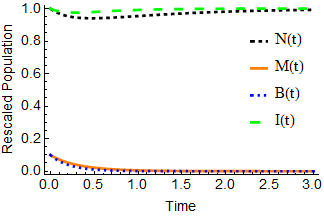
\includegraphics[width=3.2in]{1a.png}
  \caption{(Stable Equilibrium)  $\hat{j}=2$.}
  \label{F1}
\end{subfigure}%
\begin{subfigure}{.49\textwidth}
  \centering
  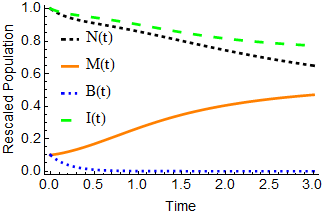
\includegraphics[width=3.2in]{1b.png}
  \caption{(Unstable Equilibrium)  $\hat{j}=7\,>5=\hat{m}+\hat{n}$.}
  \label{F2}
\end{subfigure}
\caption{Common parameters for (a) and (b): $\hat{c}=3, \, \hat{d}=1,\,  \hat{e}=1,\,  \hat{f}=3, \, \hat{g}=3,\, \hat{h}=2.5,\, \hat{l}=1,\,  \hat{m}=2,\, \hat{n}=3,\, \hat{w}=3,\, \hat{p}=2, \,
\hat{q}=1,\, \hat{s}=1,\, \hat{r}=3,\, \hat{u}=3,\, \hat{v}=4.$}
%\label{fig:test}
\end{figure}

%%%%%%%%%%%%





% Can we explain what $\hat{j}$ represents? That is, What does $\hat{j}>\hat{m}+\hat{n}$ mean by?
% Why is it unstable if we still have $e<g+h$????????????????????????
%
%\begin{figure}
%\begin{center}
%\includegraphics[width=0.9\textwidth]{FIG3.png}
%\caption{(Unstable Equilibrium) A parameter set is same as stable equilibruim's parameter set in Figure \ref{F1} except $\hat{e}=5.32 \approx \hat{g}+\hat{h}=5.5\,$:
%$\hat{c}=3, \, \hat{d}=1,\,  \hat{f}=3, \, \hat{g}=3,\, \hat{h}=2.5,\,
%\hat{j}=2, \, \hat{l}=1,\,  \hat{m}=2,\, \hat{n}=3,\, \hat{w}=3,\, \hat{p}=2, \,
%\hat{q}=1,\, \hat{s}=1,\, \hat{r}=3,\, \hat{u}=3,\, \hat{v}=4$. 
%}
%\label{F3}
%\end{center}
%\end{figure}
%
%
%Figure \ref{F3} corresponds to the same parameters as Figure \ref{F1} with the exception of $\hat{e}$ which was increased to observe what happens when $\hat{e}$ approaches $\hat{g}+\hat{h}$. For this model $\hat{e}=5.32 \approx \hat{g}+\hat{h}=5.5 $. Although the metastatic cell population still converges to zero, the other cell populations all diverge from the equilibrium points, and the population of normal cells collapses to $0$.

% Again, can we add an explanation for $\hat{e}$ as well?
%
%\begin{figure}
%\begin{center}
%\includegraphics[width=0.9\textwidth]{FIG4.png}
%\caption{[Color online] An initial conditions are $N^*(0)=5$, $M^*(0)=2$, $B^*(0)=1$, $I^*(0)=2$ and  a parameter set is as follows :
%$\hat{c}=3, \, \hat{d}=1, \, \hat{e}=1, \, \hat{f}=3, \, \hat{g}=3, \, \hat{h}=2.5, \, \hat{j}=2, \, \hat{l}=1, \, \hat{m}=2, \, \hat{n}=3, \, \hat{w}=3, \, \hat{p}=2, \, \hat{q}=1, \, \hat{s}=1, \, \hat{r}=3, \, \hat{u}=3, \, \hat{v}=4$.
%}
%\label{F4}
%\end{center}
%\end{figure}
%
%In Figure \ref{F4} the initial conditions are changed to show a system that is not at healthy equilibrium. 



  
\subsection{Effects of Immunotherapy for the One Patch Model}

According to \cite{ACS}, immunotherapy is a form of cancer treatment that uses a person's immune system to combat cancer. Immunotherapy can be implemented in a couple of different ways. Some examples include inserting man-made proteins into a patient's immune system to increase performance or simply injecting more immune cells into the body. In the following discussion the one patch model is used to analyze the outcomes of adding more immune cells to a cancerous system. Figures \ref{HI1} and \ref{HI2} represent a person with a stable immune system (i.e. the healthy equilibrium is a stable point).  Figures \ref{UHI1} and \ref{UHI2} represent a person with an unstable immune system (i.e. the healthy equilibrium is an unstable point).

%\begin{figure}
%\begin{center}
%\includegraphics[width=.9\textwidth]{stablesystemwithnoimmunotherapy.png}
%\caption{[Color online] (Stable System without Immunotherapy) A parameter set is as follows: $\hat{c}=3, \, \hat{d}=1, \, \hat{e}=2, \, \hat{f}=3, \, \hat{g}=3, \, \hat{l}=1, \, \hat{p}=2, \, \hat{r}=1.27, \, \hat{q}=1, \, \hat{s}=1, \, \hat{n}=3, \, \hat{v}=4, \, \hat{h}=2.5, \, \hat{J}=3.7, \, \hat{m}=2, \, \hat{n}=3, $ and initial conditions are $N(0)=5, \, I(0)=2, \, M(0)=2,$ and $B(0)=1$.}
%\label{HI1}
%\end{center}
%\end{figure}

Figure \ref{HI1} represents a cancerous system where the metastatic cells level off at a significant number, indicating an unhealthy state. The normal cell population is decreasing because of their competition with the metastatic and benign cells. The immune cell population is decreasing because they are dying from fighting the growing population of metastatic and benign cells. The benign cells die out because of the competition with the metastatic cells.  In order to try to drive the system to a healthy state, immunotherapy  is introduced the moment when the metastatic cells begin to out-compete the population of normal or immune cells. From the parameters we used, immunotherapy would be most effective if it were added around the time 4.5-4.8.


Figure \ref{HI2} shows that if immunotherapy is added to a cancerous system when the metastatic cell population is surpassing the growth of the other cells, the addition of more immune cells will cause the population of the metastatic cells to decrease and cause the normal cell population to grow.  In this figure the initial value of immune cells is increased so that they can fight the metastatic cells in a more aggressive manner. We can see that as time progresses, the metastatic cell population does not return; thus, this patient is cancer free. We also observe that the normal and immune cell populations reach a healthy equilibrium.

%%%%%%%%%%%%
\begin{figure}
\centering
\begin{subfigure}{.45\textwidth}
  \centering
  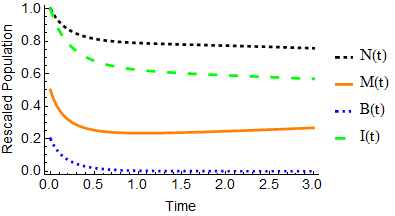
\includegraphics[width=3.3in]{2a.png}
  \caption{(Stable System without Immunotherapy) Initial conditions are $N(0)=1, \, I(0)=1, \, M(0)=0.5,$ and $B(0)=0.5$.}
  \label{HI1}
\end{subfigure}%
\hfill
\begin{subfigure}{.45\textwidth}
  \centering
  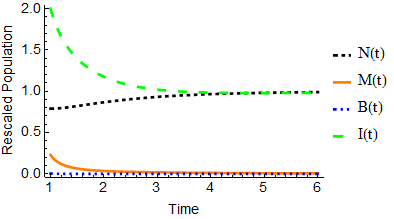
\includegraphics[width=3.3in]{2b.png}
  \caption{(Stable System with Immunotherapy) Initial conditions are $N(1)=0.79, \, I(1)=2, \, M(1)=0.23,$ and $B(1)=0.003$.}
  \label{HI2}
\end{subfigure}
\caption{Common parameters for (a) and (b):  $\hat{c}=3, \, \hat{d}=1, \, \hat{e}=2, \, \hat{f}=3, \, \hat{g}=3, \, \hat{l}=1, \, \hat{p}=2, \, \hat{r}=1.27, \, \hat{q}=1, \, \hat{s}=1, \, \hat{n}=3, \, \hat{v}=4, \, \hat{h}=2.5, \, \hat{j}=4.5, \, \hat{m}=2, \, \hat{n}=3, \, \hat{w}=1, \, \hat{u}=3$.}
%\label{fig:test}
\end{figure}

%%%%%%%%%%%%



%
%
%
%\begin{figure}
%\begin{center}
%\includegraphics[width=0.9\textwidth]{stablesystemwithimmunotherapy.png}
%\caption{[Color online] (Stable System with Immunotherapy) A parameter set is as follows: $\hat{c}=3, \, \hat{d}=1, \, \hat{e}=2, \, \hat{f}=3, \, \hat{g}=3, \, \hat{l}=1, \, \hat{p}=2, \, \hat{r}=1.27, \, \hat{q}=1, \, \hat{s}=1, \, \hat{n}=3, \, \hat{v}=4, \, \hat{h}=2.5, \, \hat{J}=3.7, \, \hat{m}=2, \, \hat{n}=3$ and initial conditions are $N(0)=5, \, I(0)=100, \, M(0)=2,$ and $B(0)=1$.}
%\label{HI2}
%\end{center}
%\end{figure}



Similarly to Figure \ref{HI1}, Figure \ref{UHI1} represents a cancerous system where the metastatic cell population surpasses the populations of normal and immune cells. However, in this case, the parameters do not satisfy conditions (\ref{nec_suf_stability}), i.e., the healthy equilibrium is unstable.

Figure \ref{UHI2} represents immunotherapy where more immune cells are added to our initial immune cell population.  Initially, the metastatic cell population looks like it is approaching zero and the population of normal cells decreases then levels off. Eventually, however, the metastatic cell population returns.  Even with the help of immunotherapy, eventually the normal cells will die out, implying that the person has died.

%%%%%%%%%%%%
\begin{figure}
\centering
\begin{subfigure}{.45\textwidth}
  \centering
  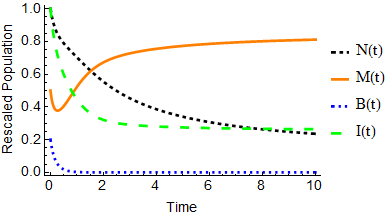
\includegraphics[width=3.3in]{3a.png}
  \caption{(Unstable System without Immunotherapy) Initial conditions are $N(0)=1, \, I(0)=1, \, M(0)=0.5,$ and  $B(0)=0.2$.}
  \label{UHI1}
\end{subfigure}%
\hfill
\begin{subfigure}{.45\textwidth}
  \centering
  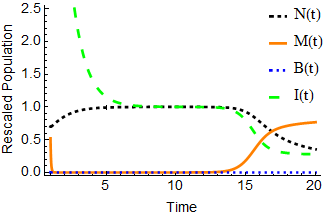
\includegraphics[width=3.0in]{3b.png}
  \caption{(Unstable System with Immunotherapy) Initial conditions are $N(1)=0.7, \, I(1)=10, \, M(1)=0.52,$ and $B(1)=0.002$.}
  \label{UHI2}
\end{subfigure}
\caption{Common parameters for (a) and (b):  $\hat{c}=3, \, \hat{d}=1, \, \hat{e}=2, \, \hat{f}=3, \, \hat{g}=3, \, \hat{l}=1, \, \hat{p}=2, \, \hat{r}=1, \, \hat{q}=1, \, \hat{s}=1, \, \hat{n}=3, \, \hat{v}=4, \, \hat{h}=2.5, \, \hat{j}=6.7, \, \hat{m}=2, \, \hat{w}=1, \, \hat{w}=3$.}
%\label{fig:test}
\end{figure}

%%%%%%%%%%%%

%\begin{figure}
%\begin{center}
%\includegraphics[width=0.9\textwidth]{unstablesystemwithnoimmunotherapy.png}
%\caption{[Color online] (Unstable System without Immunotherapy) A parameter set is as follows: $\hat{c}=3, \, \hat{d}=1, \, \hat{e}=2, \, \hat{f}=3, \, \hat{g}=3, \, \hat{l}=1, \, \hat{p}=2, \, \hat{r}=1, \, \hat{q}=1, \, \hat{s}=1, \, \hat{n}=3, \, \hat{v}=4, \, \hat{h}=2.5, \, \hat{j}=6.7, \, \hat{m}=2, \, \hat{n}=3$ and initial conditions are $N(0)=5, \, I(0)=2, \, M(0)=2,$ and  $B(0)=1$.}
%\label{UHI1}
%\end{center}
%\end{figure}
%
%
%
%\begin{figure}
%\begin{center} 
%\includegraphics[width=0.9\textwidth]{unstablesystemwithimmunotherapy.png}
%\caption{[Color online] (Unstable System with Immunotherapy) A parameter set is as follows: $\hat{c}=3, \, \hat{d}=1, \, \hat{e}=2, \, \hat{f}=3, \, \hat{g}=3, \, \hat{l}=1, \, \hat{p}=2, \, \hat{r}=1, \, \hat{q}=1, \, \hat{s}=1, \, \hat{n}=3, \, \hat{v}=4, \, \hat{h}=2.5, \, \hat{j}=6.7, \, \hat{m}=2, \, \hat{n}=3$ and initial conditions are $N(0)=5, \, I(0)=100 , \, M(0)=2,$ and $B(0)=1$.}
%\label{UHI2}
%\end{center}
%\end{figure}



According to \cite{MD}, for 2 women out of 9 with cervical cancer, the cancer went away and for the remaining 7 it either came back or never went away. While exploring how effective immunotherapy would be with our models, we can conclude that it depends on the person's immune system and whether the healthy equilibrium  is stable or unstable (i.e., whether conditions (\ref{nec_suf_stability}) are satisfied or not). We believe that this could help explain why immunotherapy  works for some individuals and not for others.  Hopefully immunotherapy in addition to other methods of fighting cancer, such as chemotherapy, could possibly help an unstable immune system eradicate cancer. This is something we intend to study further in the future.


\section{Two Patch Model}

For our two patch model, we assume that metastatic cells and immune cells are mobile. To account for this we have added migration terms $\mu_i$ and $\gamma_i$, where $i=1,2$ represent the two patches. When $\mu_i$ is negative it denotes a migration out of patch $i$ and a positive $\mu_i$ denotes a migration into patch $i$. The same applies to a positive or negative $\gamma_i$. There is one equation for each type of cell and each patch contains all four cell types; so, there are eight  equations altogether. The following is the ODE system for two patches:
\begin{eqnarray}
N_1' &=& a_1N_1-b_1a_1N_1^2-c_1B_1N_1-d_1M_1N_1,\label{normal1}\nonumber\\
N_2' &=&a_2N_2-b_2a_2N_2^2-c_2B_2N_2-d_2M_2N_2,\label{normal2}\nonumber\\
B_1' &=&e_1B_1(1-\frac{B_1}{K_1}-\frac{f_1M_1}{K_1})-\frac{g_1B_1N_1}{K_1}-h_1B_1I_1,\label{benign1}\nonumber\\
B_2' &=& e_2B_2(1-\frac{B_2}{K_2}-\frac{f_2M_2}{K_2})-\frac{g_2B_2N_2}{K_2}-h_2B_2I_2,\label{benign2}\nonumber\\
M_1' &=&j_1M_1(1-\frac{M_1}{K_3}-\frac{l_1B_1}{K_3})-\frac{m_1M_1N_1}{K_3}-n_1M_1I_1-\mu _1M_1+ \mu _2M_2,\label{metastatic1}\nonumber\\
M_2' &=& j _2M_2(1-\frac{M_2}{K_4}-\frac{l_2 B_2}{K_4})-\frac{m_2M_2N_2}{K_4}-n_2M_2N_2-\mu _2M_2+ \mu _1M_1,\label{metastatic2}\nonumber\\
I_1' &=& o+\frac{p _1I_1B_1}{q_1+B_1}+\frac{r_1I_1M_1}{s_1+M_1}-u_1I_1B_1-v_1I_1M_1-w_1I_1-\gamma _1I_1+\gamma _2I_2,\label{immune1}\nonumber\\
I_2' &=& o+\frac{p _2I_2B_2}{q_2+B_2}+\frac{r_2I_2M_2}{s_2+M_2}-u_2I_2B_2-v_2I_2M_2-w_2I_2-\gamma _2I_2+\gamma_1I_1,\label{immune2}.\nonumber
\end{eqnarray}
The equations in the two patch model are very similar to those used in the one patch model. New additions to the two patch model include the subscripts 1 and 2 to denote which patch each variable is referring to and migration rates represented by terms at the end of the metastatic and immune cell equations to account for the cells'  ability to move between the two patches.

\subsection{Nondimensionalization}

Similarly to the one patch model, we nondimensionalized the equations for the two patch model. This resulted in the following change of variables
\begin{equation*}
\begin{array}{ccccc}
N_1=\dfrac{N_1^*}{b_1}, & B_1=B_1^*K_1, & M_1=M_1^*K_3, & I_1=\dfrac{I_1^*o}{w_1}, & N_2=\dfrac{N_2^*}{b_2},\\
B_2=B_2^*K_2, & M_2=M_2^*K_4, & I_2=\dfrac{I_2^*o}{w_2}, & t=\dfrac{t^{*}}{a_1}, &
\end{array}
\end{equation*}
where the starred quantities are nondimensional. For convenience, we set 
\begin{equation*}
\begin{array}{llllll}
\hat{c_1}=\dfrac{c_1K_1}{a_1}, & \hat{d_1}=\dfrac{d_1K_3}{a_1}, & \hat{a_2}=\dfrac{a_2}{a_1}, & \hat{c_2}=\dfrac{c_2K_2}{a_1}, & \hat{d_2}=\dfrac{d_2 K_4}{a_1}, & \hat{e_1}=\dfrac{e_1}{a_1},       \\
\hat{f_1}=\dfrac{f_1K_3}{K_1}, & \hat{g_1}=\dfrac{g_1}{a_1b_1K_1}, & \hat{h_1}=\dfrac{h_1o}{w_1a_1}, & \hat{e_2}=\dfrac{e_2}{a_1}, & \hat{f_2}=\dfrac{f_2 K_4}{K_2}, & \hat{g_2}=\dfrac{g_2}{b_2K_2a_1},      \\
\hat{h_2}=\dfrac{h_2o}{w_2a_1}, & \hat{j_1}=\dfrac{j_1}{a_1}, & \hat{l_1}=\dfrac{l_1K_1}{K_3}, & \hat{m_1}=\dfrac{m_1}{a_1b_1K_3}, & \hat{n_1}=\dfrac{n_1o}{w_1a_1}, & \hat{\mu_1}=\dfrac{\mu_1}{a_1},       \\
\hat{\mu_2}=\dfrac{\mu_2}{a_1}, & \hat{\alpha}=\dfrac{K_4}{K_3}, & \hat{j_2}=\dfrac{j_2}{a_1}, & \hat{l_2}=\dfrac{l_2K_2}{K_4}, & \hat{m_2}=\dfrac{m_2}{a_1K_4b_2}, & \hat{n_2}=\dfrac{n_2o}{w_2a_1},       \\
\hat{w_1}=\dfrac{w_1}{a_1}, & \hat{p_1}=\dfrac{p_1}{a_1}, & \hat{q_1}=\dfrac{q_1}{K_1}, & \hat{r_1}=\dfrac{r_1}{a_1}, & \hat{s_1}=\dfrac{s_1}{K_3}, & \hat{u_1}=\dfrac{u_1K_1}{a_1},       \\
\hat{v_1}=\dfrac{v_1K_3}{a_1}, & \hat{\gamma_1}=\dfrac{\gamma_1}{a_1}, & \hat{\gamma_2}=\dfrac{\gamma_2}{a_1}, & \hat{\beta}=\dfrac{w_1}{w_2}, & \hat{w_2}=\dfrac{w_2}{a_1}, & \hat{p_2}=\dfrac{p_2}{a_1},       \\
\hat{q_2}=\dfrac{q_2}{K_2}, & \hat{r_2}=\dfrac{r_2}{a_1}, & \hat{s_2}=\dfrac{s_2}{K_4}, & \hat{u_2}=\dfrac{u_2K_2}{a_1}, & \hat{v_2}=\dfrac{v_2K_4}{a_1}.
\end{array}
\end{equation*}
Thus, the ODE system of  nondimensionalized equations takes the following form:
\begin{eqnarray}
\dfrac{dN_1^*}{dt^*}&=&N_1^* - (N_1^*)^2 - \hat{c_1}B_1^*N_1^*-\hat{d_1}M_1^*N_1^*, \label{N_1^*}\\
\dfrac{dN_2^*}{dt^*}&=&\hat{a_2}N_2^* -\hat{a_2} (N_2^*)^2 - \hat{c_2}B_2^*N_2^*-\hat{d_2}M_2^*N_2^*, \label{N_2^*}\\
\dfrac{dB_1^*}{dt^*}&=&\hat{e_1}B_1^*(1-B_1^*-\hat{f_1}M_1^*)-\hat{g_1}B_1^*N_1^*-\hat{h_1}B_1^*I_1^*, \label{B_1^*}\\
\dfrac{dB_2^*}{dt^*}&=&\hat{e_2}B_2^*(1-B_2^*-\hat{f_2}M_2^*)-\hat{g_2}B_2^*N_2^*-\hat{h_2}B_2^*I_2^*, \label{B_2^*}\\
\dfrac{dM_1^*}{dt^*}&=&\hat{j_1}M_1^*(1-M_1^*-\hat{l_1}B_1^*)-\hat{m_1}M_1^*N_1^*- \hat{n_1}M_1^*I_1^*-\hat{\mu_1}M_1^*+\hat{\mu_2}\hat{\alpha}M_2^*, \label{M_1^*}\\
\dfrac{dM_2^*}{dt^*}&=&\hat{j_2}M_2^*(1-M_2^*-\hat{l_2}B_2^*)-\hat{m_2}M_2^*N_2^*-\hat{n_2}M_2^*I_2^*-\hat{\mu_2}M_2^*+ \dfrac{\hat{\mu_1}}{\hat{\alpha}}M_1^*, \label{M_2^*}\\
\dfrac{dI_1^*}{dt^*}&=&\hat{w_1}+\dfrac{\hat{p_1}I_1^*B_1^*}{\hat{q_1}+B_1^*}+\dfrac{\hat{r_1}I_1^*M_1^*}{\hat{s_1}+M_1^*}-\hat{u_1}I_1^*B_1^*-\hat{v_1}I_1^*M_1^*-\hat{w_1}I_1^*- \hat{\gamma_1}I_1^*+\hat{\gamma_2}\hat{\beta}I_2^*, \label{I_1^*}\\
\dfrac{dI_2^*}{dt^*}&=&\hat{w_2}+\dfrac{\hat{p_2}I_2^*B_2^*}{\hat{q_2}+B_2^*}+\dfrac{\hat{r_2}I_2^*M_2^*}{\hat{s_2}+M_2^*}-\hat{u_2}I_2^*B_2^*-\hat{v_2}I_2^*M_2^*-\hat{w_2}I_2^*- \hat{\gamma_2}I_2^*+\dfrac{\hat{\gamma_1}}{\hat{\beta}}I_1^*. \label{I_2^*}
\end{eqnarray}
The above system of equations is used to find a healthy equilibrium point for the two patch model. A healthy equilibrium is again defined as having some normal and immune cells in each patch and no tumor cells. So, $B_1^*, B_2^*, M_1^*,$ and $M_2^*$ all equal zero. This makes equations (\ref{B_1^*}), (\ref{B_2^*}), (\ref{M_1^*}), and (\ref{M_2^*}) trivially satisfied. The remaining equations are set equal to zero and we solve for $N_1^*, N_2^*, I_1^*,$ and $I_2^*$. Equations (\ref{N_1^*}) and (\ref{N_2^*}) are simple and result in $N_1^*=1$ and $N_2^*=1$. Equations (\ref{I_1^*}) and (\ref{I_2^*}) are more complicated and simplify in the following manner
\begin{equation*}
I_1^* = \dfrac{\hat{w}_1+\hat{\gamma}_2\hat{\beta}I_2^*}{\hat{w}_1+\hat{\gamma}_1}, \qquad
I_2^* = \dfrac{\hat{w}_2+\frac{\hat{\gamma}_1}{\hat{\beta}}I_1^*}{\hat{w}_2+\hat{\gamma}_2}.
\end{equation*}
After substitution we obtained
\begin{equation*}
I_1^* = \dfrac{\hat{w}_1\hat{w}_2+\hat{w}_1\hat{\gamma}_2+\hat{\gamma}_2\hat{\beta}\hat{w}_2}{\hat{w}_1\hat{w}_2+\hat{w}_2\hat{\gamma}_1+\hat{w}_1\hat{\gamma}_2}, \qquad 
I_2^* = \dfrac{\hat{w}_1\hat{w}_2\hat{\beta}+\hat{w}_2\hat{\gamma}_1\hat{\beta}+\hat{w}_1\hat{\gamma}_1}{\hat{\beta}(\hat{w}_1\hat{w}_2+\hat{w}_1\hat{\gamma}_2+\hat{w}_2\hat{\gamma}_1)}.
\end{equation*}
From now we will denote these values $I_1^*$ and $I_2^*$ by $w_1^*$ and $w_2^*$ respectively. Thus, the healthy equilibrium point for the two patch model is $(N_1^*N_2^*, B_1^*, B_2^*, M_1^*, M_2^*, I_1^*, I_2^*) = (1, 1, 0, 0, 0, 0, w_1^*, w_2^*)$.

\subsection{Determining Stability of Healthy Equilibrium Point $(1, 1, 0, 0, 0, 0, w_1^*, w_2^*)$}

We use methods very similar to those used in our analysis of the healthy equilibrium point for the one patch model to determine the stability of this equilibrium point. After linearizing the system equations (\ref{N_1^*}-\ref{I_2^*}) about the point $(N_1^*N_2^*, B_1^*, B_2^*, M_1^*, M_2^*, I_1^*, I_2^*) = (1, 1, 0, 0, 0, 0, w_1^*, w_2^*)$, we arrive at
\begin{eqnarray}
\hat{N_1}'&=&-\hat{N_1}-\hat{c_1}\hat{B}-\hat{d_1}\hat{M_1}, \nonumber\\
\hat{N_2}'&=&-\hat{a_2}\hat{N_2}-\hat{c_2}\hat{B_2}-\hat{d_2}\hat{M_2}, \nonumber\\
\hat{B_1}'&=&e_1^*\hat{B_1}, \nonumber\\
\hat{B_2}'&=&e_2^*\hat{B_2}, \nonumber\\
\hat{M_1}'&=&j_1^*\hat{M_1}+\hat{\mu _2^*}\hat{M_2}, \nonumber\\
\hat{M_2}'&=&\mu _1^*\hat{M_1}+j_2^*\hat{M_2}, \nonumber\\
\hat{I_1}'&=&p_1^*\hat{B_1}+r_1^*\hat{M_1}-\gamma _1^*\hat{I_1}+\gamma _2^*\hat{I_2}, \nonumber\\
\hat{I_2}'&=&p_2^*\hat{B_2}+r_2^*\hat{M_2}+\phi _1^*\hat{I_1}-\phi _2^*\hat{I_2},\nonumber
\end{eqnarray}
where $e_1^*=\hat{e_1}-\hat{g_1}-\hat{h_1}w_1^*$,  $e_2^*=\hat{e_2}-\hat{g_2}-\hat{h_2}w_2^*$, $j_1^*=\hat{j_1}-\hat{m_1}-\hat{n_1}w_1^*-\hat{\mu _1}$, $\mu _2^*=\hat{\mu _2}\hat{\alpha}$,  $j_2^*=\hat{j_2}-\hat{m_2}-\hat{n_2}w_2^*-\hat{\mu _2}$, $\mu _1^*=\dfrac{\hat{\mu _1}}{\hat{\alpha}}$, $p_1^*=\dfrac{\hat{p_1}w_1^*}{\hat{q_1}}-\hat{u_1}w_1^*$,  $r_1^*=\dfrac{\hat{r_1}w_1^*}{\hat{s_1}}-\hat{v_1}w_1^*$, $\gamma _1^*=\hat{w_1}-\hat{\gamma _1}$, $\gamma _2^*=\hat{\gamma _2}\hat{\beta}$, $p_2^*=\dfrac{\hat{p_2}w_2^*}{\hat{q_2}}-\hat{u_2}w_2^*$, $r_2^*=\frac{\hat{r_2}w_2^*}{\hat{s_2}}-\hat{v_2}w_2^*$,  $\phi _1^*=\frac{\gamma _1}{\hat{\beta}}$, and $\phi _2^*=\hat{w_2}+\hat{\gamma _2}$.

One can easily show that the eigenvalues associated with the above system of equations are given by
\begin{eqnarray}
&&\lambda_1 =-1, \lambda_2 = -\hat{a}_2, \lambda_3 = e_1^*, \lambda_4 = e_2^*, \nonumber\\
\lambda_5 &=& \dfrac{1}{2}(-\gamma_1^* + \phi_2^* - \sqrt{(\gamma_1^*)^2 + 2\gamma_1^*\phi_2^* + (\phi_2^*)^2 + 4\gamma_2^*\phi_1^*}), \nonumber\\
\lambda_6 &=& \dfrac{1}{2}(-\gamma_1^* + \phi_2^* + \sqrt{(\gamma_1^*)^2 + 2\gamma_1^*\phi_2^* + (\phi_2^*)^2 + 4\gamma_2^*\phi_1^*}), \nonumber\\
\lambda_7 &=& \dfrac{1}{2}(j_1^* + j_2^* - \sqrt{(j_1^*)^2 - 2j_1^*j_2^* + (j_2^*)^2 + 4\mu_1^*\mu_2^*}), \nonumber\\
\lambda_8 &=& \dfrac{1}{2}(j_1^* + j_2^* + \sqrt{(j_1^*)^2 - 2j_1^*j_2^* + (j_2^*)^2 + 4\mu_1^*\mu_2^*}).\nonumber
\end{eqnarray}
 As discussed above, the healthy equilibrium point is asymptotically stable if and only if $\lambda_i<0$ for all $i=1,\dots 8$. Similarly to the one patch model, the stability of the healthy equilibrium point depends on the birth rate of the benign and metastatic cells and the rate at which they compete with normal cells and are killed by immune cells.


%%% Don't you have any numerical simulations for two patch model?


\section{Discussion}

We  based our analysis on mathematical models of cancer introduced in  \cite{DEPILLIS}, where three types of cells were considered: normal, tumor, and immune cells. In our model, however, the tumor cell population is split into two different types of cells - metastatic and benign, thus arriving to what we refer to as the ``one patch model". Necessary and sufficient conditions for the stability of the healthy equilibrium point were derived analytically and studied numerically. Further, the effects of immunotherapy were studied, both in the case of a stable healthy equilibrium and in the case of an unstable one. In the former case, a person's tumor cell population can be eradicated using immunotherapy, while in the latter case, after an initial decline in the tumor population, the metastatic tumor cells can come back. Furthermore, in order to capture the effects of cell migration, the two patch model was created and necessary and sufficient conditions for stability of the healthy equilibrium point were derived. 

For future investigations,  a more in depth biological background  could help with a more accurate  choice of the parameters for the numerical experiments.  An understanding of how cancer moves in the body can assist in finding ways to control aspects, such as metastatic cell mobility and the rapid growth rates of the benign and metastatic cell populations, which make cancer such a lethal disease. 

\begin{thebibliography}{cc}

\bibitem{ACS} American Cancer Society, \emph{What is Cancer Immunotherapy?} American Cancer Society %\url{http://www.cancer.org/treatment/treatmentsandsideeffects/treatmenttypes/immunotherapy/immunotherapy-what-is-immunotherapy}
%March 26, 2014. June 2, 2014.

\bibitem{MD} Sabrina Bachai, \emph{Immunotherapy Could Offer Lifelong Cure To Terminally Ill Cervical Cancer Patients}. Medical Daily %\url{http://www.medicaldaily.com/immunotherapy-could-offer-lifelong-cure-terminally-ill-cervical-cancer-patients-285914}
% June 2, 2014.

\bibitem{DEPILLIS} L.G. DePillis, A. Radunskaya, \emph{The Dynamics of an Optimally Controlled Tumor Model: A Case Study}. Elsevier Science Ltd.
(2003).

\bibitem{GABRIEL} Janice Gabriel, \emph{The Biology of Cancer}. John Wiley \& Sons, Ltd.
(2007).

\bibitem{ITIK} Mehmet Itik, Metin U. Salamci, Stephen P. Banks, \emph{Optimal Control of Drug Therapy in Cancer Treatment}. Elsevier Ltd.
(2009).

\bibitem{NIH} U.S. Department of Health and Human Services, National Institutes of Health, \emph{Understanding the Immune System: How It Works}. National Institute of Allergy and Infectious Diseases
(2007).



\end{thebibliography}




\end{document}
